% Copyright 2022 Thomas Ascher
% SPDX-License-Identifier: CC-BY-SA-4.0

\documentclass[a4paper,parskip=half]{scrartcl}

\usepackage[T1]{fontenc}
\usepackage{mathpazo}
\usepackage[naustrian]{babel}
\usepackage{csquotes}
\usepackage{booktabs}
\usepackage{graphicx}
\usepackage{chemformula}
\usepackage{icomma}
\usepackage{gensymb}
\usepackage{float}
\usepackage[section]{placeins}
\usepackage[style=apa,backend=biber]{biblatex}

\usepackage[hidelinks,pdfencoding=auto,
  pdfauthor={Thomas Ascher},
  pdfusetitle,
  pdfkeywords={Bier,Bitterung,Bitterstoffausbeute,IBU,Tinseth,Rager,Garetz}]{hyperref}
\usepackage{microtype}
%\DisableLigatures{encoding=*, family=*}

\setkomafont{disposition}{\normalfont\bfseries}

\addto\extrasnaustrian{
\def\figureautorefname{Abb.}
\def\tableautorefname{Tab.}
\def\equationautorefname{Gl.}
}

\addto\captionsnaustrian{
\renewcommand{\figurename}{Abb.}
\renewcommand{\tablename}{Tab.}
}

\NewBibliographyString{gethesis}
\DefineBibliographyStrings{naustrian}{
  mathesis = {Masterarbeit},
  gethesis = {Diplomarbeit},
}

\newcommand{\BA}{\mathit{BA}}
\newcommand{\BAKt}{{\mathit{BA}}_{\mathit{Kd}}}
\newcommand{\IBU}{\mathit{IBU}}
\newcommand{\umin}{\:[\textrm{min}]}
\newcommand{\uden}{\:[\text{g/cm³}]}
\newcommand{\uper}{\:[\text{\%}]}
\newcommand{\uli}{\:[\text{l}]}
\newcommand{\ume}{\:[\text{m}]}
\newcommand{\ucon}{\:[\text{mg/l}]}
\newcommand{\FKd}{F_{\mathit{d}}}
\newcommand{\FHR}{F_{\mathit{KA}}}
\newcommand{\FSP}{F_{\mathit{SW}}}
\newcommand{\FAH}{F_{\mathit{SH}}}
\newcommand{\FHF}{F_{\mathit{HP}}}
\newcommand{\FHS}{F_{\mathit{HS}}}
\newcommand{\FFil}{F_{\mathit{FI}}}
\newcommand{\dPfvw}{d_\mathit{Pfvw}}
\newcommand{\dKt}{\overline{d_{\mathit{Kd}}}}

\title{Eine bittere Angelegenheit: Historische IBU Berechnungen}
\author{Thomas Ascher <thomas.ascher@gmx.at>}
\date{\today, \href{http://creativecommons.org/licenses/by-sa/4.0/}{CC BY-SA 4.0}}

\addbibresource{hopfenbittere.bib}

\begin{document}
\maketitle

\section*{Einleitung}

Die Einstellung des durch Hopfen eingebrachten Bitterstoffgehalts eines Biers, den wir als IBU-Angabe kennen, ist ein wesentlicher Bestandteil des Brauprozesses und der Rezeptentwicklung. Typischerweise helfen uns heute Braurechner bei der Bestimmung von benötigten Hopfenmengen. Aber wie funktionieren deren Berechnungen? Dieser Artikel soll darüber Aufschluss geben und stellt historische Berechnungsverfahren aus dem Heimbraubereich vor.

\section*{Bitterstoffe und die International Bitterness Unit}

Die vorrangigen Bitterstoffe im Bier sind die Isomere der Alphasäuren des Hopfens: Isohumulone, Isocohumulone und Isoadhumulone. Darüber hinaus tragen auch noch weitere Hopfenbestandteile zum Bittereindruck bei, insbesondere Oxidationsprodukte der Alpha- und Betasäuren. \parencite{MEBAK2020}

Für die Bildung der Weichharze, zu denen Alpha- und Betasäuren (Lupulone, Colupulone und Adlupulone) zählen, sind die Lupulindrüsen in den Dolden der weiblichen Hopfenpflanzen zuständig. Nicht oxidierte Weichharze sind weder in der Würze noch im Bier bei Raumtemperatur gut löslich. Die Alphasäuren durchlaufen jedoch während des Hopfenkochens einen Isomerisierungsprozess, eine molekulare strukturelle Veränderung und bilden die Isoalphasäuren, welche in der Lösung verbleiben. \parencites{Hall1997}[20-23]{Nottebohm2020}

Die Kennzahl zur Beschreibung des sensorischen Bittereindrucks eines Biers ist die International Bitterness Unit (IBU). In der deutschsprachigen Fachliteratur wird alternativ auch die Bezeichnung Bittereinheiten (BE) verwendet. Eine IBU entspricht einer Konzentration von einem Milligramm Isoalphasäure pro Liter Bier. Bei stark und kalt gehopften Bieren lässt sich der sensorische Bittereindruck durch vermehrt eingebrachte oxidierte Hopfenbestandteile und Polyphenole nicht mehr ausreichend durch die IBU charakterisieren. Die Schaffung neuer Wahrnehmungsmodelle, die unter anderem neben den Isoalphasäurekonzentration auch Oxidationsprodukte und den Alkoholgehalt berücksichtigen, sind Gegenstand aktueller Forschung. \parencite{Kishimoto2021}

Von normgebenden Gremien der Brauindsutrie – der \href{https://www.asbcnet.org}{ASBC}, der \href{https://europeanbreweryconvention.eu}{EBC} und der \href{https://www.mebak.org}{MEBAK} – wurde zur Messung der IBU ein in den 1950er-Jahren entwickeltes, kostengünstiges, spektralphotometrisches, analytisches Verfahren ratifiziert. Dabei erfolgt keine direkte Messung der Isoalphasäurekonzentration, sondern eine Korrelation der gemessenen Lichtabsorption einer aufbereiteten Bierprobe bei einer Wellenlänge von 275~nm. Es absorbieren aber auch andere Bestandteile der Probe Licht in diesem Spektrum. Die angewendete Korrelation, die Multiplikation des Messwertes mit 50, ist allerdings nur für typische Biere der 1950er und 1960er-Jahre gültig, da heute eingesetzter Hopfen aufgrund besserer Lagerbedingungen weniger Oxidationsprodukte enthält. Die derzeit genaueste
verfügbare Messmethode basiert auf der Hochleistungsflüssigkeitschromatographie (HPLC),
bei der sich Einzelververbindungen spezifisch messen lassen. Die Problematik der spektralphotometrischen Methode kann somit vermieden werden. \parencites{ASBC2011}{Hosom2017}[28]{Nottebohm2020}

Die Anschaffungskosten für Spektralphotometer und HPLC-Apparaturen sind für Privatpersonen nur schwer zu decken. \textcite{Calado2019} haben aber eine kostengünstige, auf Fluoreszenz basierende, Messmethode unter dem Einsatz einer UV-LED, einer Digitalkamera und Bildverarbeitungsalgorithmen vorgeschlagen, die eine mittlere quadratische Abweichung von 3~IBU im Vergleich zur Messung mit einem Spektralphotometer erreicht. Darüber hinaus bieten einige Labore, wie „\href{https://bieranalyse.de}{Bieranalyse Fuchs}“ und „\href{https://www.weinlabor-krauss.de}{Weinlabor Krauß}“, Messdienste für Privatpersonen an.

\section*{Bitterstoffausbeute}

Nur etwa 10 bis 40~\% der dosierten Alphasäuremenge gelangt als Isoalphasäure in ein fertiges Bier. Der genaue Prozentsatz ist dabei unter anderem davon abhängig, wie viel Alphasäure aus dem eingesetzten Hopfenprodukt extrahiert werden kann, wie vollständig die Isomerisierung verläuft und wie viele Bitterstoffe durch Trubbildung, Filterung und Gärung verloren gehen. Hopfen verliert auch durch Oxidation bei längerer Lagerung zunehmend an Alphasäure. Der zu erwartende Verlust ist sortenabhängig und wird über den Hop Storage Index (HSI) quantifiziert, der sich messtechnisch bestimmen lässt. \parencites[9]{Malowicki2005}[103\psq]{Garetz1994} 

Der Prozessparameter, der beschreibt, wie effektiv Bitterstoffe verwertet werden, heißt Bitterstoffausbeute (BA) und ist gemäß \autoref{eq:badef}, basierend auf dem Verhältnis zwischen den in einem Bier enthaltenen Bittereinheiten und der in der Pfannenvollwürze (Pfvw; vor dem Hopfenkochen) dosierten Alphasäure, definiert. Die Bitterstoffausbeute lässt sich alternativ auch hinsichtlich der Anstellwürze statt dem fertigen Bier spezifizieren. Dabei sind aber keine Gärungsverluste berücksichtigt. \parencite[163]{Annemueller2015} 

\begin{equation}
\BA \uper = \frac{\text{Isohumulongehalt des Bieres [IBU]}}{\text{Alphasäuredosierung in kalter Pfvw} \ucon} \cdot 100
\label{eq:badef}
\end{equation}

Sind die Bitterstoffausbeute und der Alphasäuregehalt eines Hopfens bekannt, so können für eine Hopfengabe die resultierenden Bittereinheiten durch \autoref{eq:ibucalc} bestimmt werden \parencite{Thesseling2019}. Es ist möglich, Hopfengaben zusammenzustellen, die rechnerisch in Summe 100 IBU überschreiten. Die hier zugrunde liegenden chemischen Reaktionen beim Hopfenkochen sind dabei aber ein limitierender Faktor \parencite{Deutschman2017}.

\begin{equation}
\IBU \ucon = \frac{\text{Hopfenmenge [mg]} \cdot \frac{\text{Alphasäuregehalt} \uper}{100} \cdot \frac{\BA \uper}{100}}{\text{Volumen kalte Anstellwürze} \uli}
\label{eq:ibucalc}
\end{equation}

Folgende Faktoren begünstigen die Bitterstoffausbeute: längere Kochdauer, höhere Kochtemperaturen, höherer Zerkleinerungsgrad des Hopfens, geringere Alphasäuredosierung, geringerer Extraktgehalt in der Würze, geringere Trubbildung und schnellere Ausflockung der Hefe \parencite{Hosom2017}. Eine Kochdauer zwischen 60 bis 90~Minuten (\autoref{fig:utiltinseth}) sind in Hinsicht auf die Hopfenausnutzung optimal \parencite[5]{Malowicki2005}. Dabei ist jedoch zu beachten, dass mit zunehmender Kochdauer Isoalphasäuren zu anderen, teilweise sensorisch unangenehmen, Produkten abgebaut werden \parencite{Kappler2010}.

\begin{figure}[H]
\centering
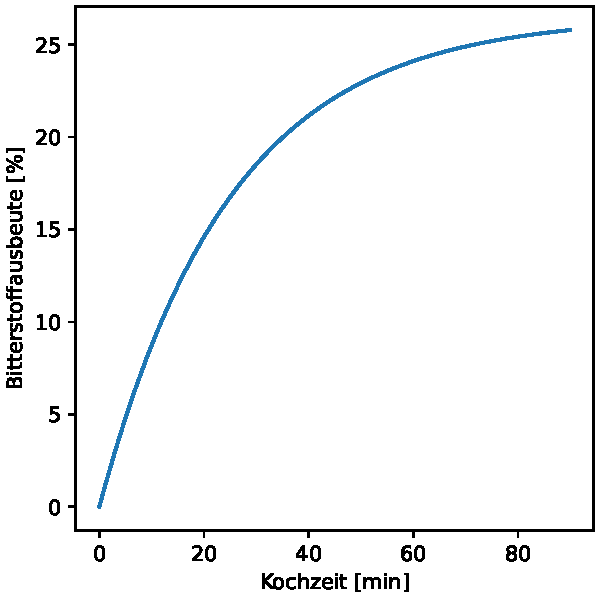
\includegraphics[width=6cm]{graph_tinseth.pdf}
\caption{Bitterstoffausbeute nach Tinseth (Ascher, 2022)}
\label{fig:utiltinseth}
\end{figure}

Während der Gärung treibt die gebildete Kohlensäure einen Teil der Isoalphasäuren aus. Ein Teil davon verfängt sich in der Hefedecke oder sammelt sich am Rand des Gärbehälters und verhärtet sich aufgrund der Oxidation. Ein weiterer Teil haftet an den Hefezellen an. Je langsamer eine Hefe ausflockt, desto mehr Bitterstoffe können an ihr anhaften und sedimentieren. Verbleibt die Hefe im Bier, so wie beim Weißbier, ist dementsprechend auch der Bitterstoffverlust geringer. \parencite[126]{Garetz1994} 

\section*{Hopfenprodukte}

Die Dolden des Hopfens werden nach der Ernte aufgrund ihrer Verderblichkeit zunächst getrocknet, konditioniert, gepresst und anschließend zu verschiedenen Endprodukten weiterverarbeitet. Ausgenommen davon ist der Grünhopfen, dessen Verwendung möglichst direkt nach der Ernte erfolgt. Eine Erhebung des Alphasäuregehalts des Grünhopfens erfolgt im Normalfall nicht. Im Heimbraubereich sind vor allem T90~Pellets, die circa aus 95~\% des ursprünglichen Pflanzenmaterials bestehen, gängig. Bei deren Herstellung werden Dolden zunächst geschreddert, gepresst und extrudiert. Das Schreddern zerstört auch die Lupulindrüsen, was beim Hopfenkochen für eine bessere Ausbeute sorgt. Wird bis zu 45~\% des ursprünglichen Pflanzenmaterials entfernt, entstehen dabei die angereicherten T45~Pellets. Es ist möglich, bei der Verarbeitung noch weiteres Pflanzenmaterial zu entfernen und somit konzentriertes Lupulinpulver zu erhalten. Dieses Endprodukt wird zum Beispiel unter den Namen Cryo Hops, Hop Hash oder Nectar vertrieben. Alternativ können Hopfenharze auch durch verschiedene Lösungsmittel aus den Dolden gelöst werden. Einige Hopfenprodukte sind ebenfalls in vorisomerisierter Form erhältlich. \parencites[166-172]{Nottebohm2020}[80-90]{Garetz1994}

\section*{Modelle zur Schätzung der Bitterstoffausbeute}

Brauereien mit der entsprechenden Laborausrüstung können die Bitterstoffausbeute messtechnisch bestimmen. Im Heimbraubereich wurden stattdessen Berechnungsmodelle auf Basis von veröffentlichten Messdaten der Brauindustrie und zum Teil von eigenen erhobenen Messdaten entwickelt, um zumindest grobe Abschätzungen der Bitterstoffausbeute treffen zu können. Dabei dürfte laut \textcite{Bonham2001} das 1986 veröffentlichte Modell von Burch eines der ersten gewesen sein. Während der Neunzigerjahre sind weitere Modelle entstanden. Von diesen hat sich schlussendlich das Tinseth Modell als De-facto-Standard etabliert \parencite[185]{Hieronymus2012}.

Zur Herstellung von hopfenaromatischen Bieren erfolgen mittlerweile größere Hopfengaben bei Kochende oder während der Whirlpoolrast. Hierbei ist zu beachten, dass bei geringeren Temperaturen als 100~°C noch eine Nachisomerisierung stattfindet \parencite{Weiss2019}. Die Modelle der Neunzigerjahre berücksichtigen diesen Effekt nicht, was bei späten Hopfengaben zu einer geringen Schätzung der Bitterstoffausbeute führt. Inzwischen wurde das Tinseth Modell bereits mehrfach erweitert, um die Nachisomerisierung zu berücksichtigen. Besonders aktiv bei der Suche nach besseren Modellen ist der Heimbrauer J.-P. Hosom mit seinem Blog „\href{https://jphosom.github.io/alchemyoverlord}{Alchemyoverlord}“, auf dem bereits das mIBU und das SMPH Modell veröffentlicht wurden \parencites{Hosom2015}{Hosom2021}.

\textcite{Hall1997} hat bereits die relevanten Modelle der Neunzigerjahre analysiert, deren Daten normalisiert und in ein gemeinsames Berechnungsschema übergeführt. Die nachfolgenden Beschreibungen enthalten jedoch die Angaben der ursprünglichen Publikationen. Bei dem allgemeinen Berechnungsschema ist pro Hopfengabe zuerst eine initiale Bitterstoffausbeute, basierend auf der Kochdauer ($\BAKt$), zu bestimmen und anschließend durch mehrere Korrekturfaktoren anzupassen. Aus den eingebrachten Alphasäuremengen der einzelnen Gaben und den ermittelten Bitterstoffausbeuten lässt sich dann ein IBU-Wert für ein Rezept berechnen. Folgende Korrekturfaktoren sind modellabhängig vorgesehen:

\begin{itemize}
\item Relative Dichte der „Kochwürze“ ($\FKd$)
\item Alphasäurekonzentration ($\FHR$)
\item Siedepunkt des Wassers basierend auf der Seehöhe ($\FSP$)
\item Sedimentationsverhalten der Hefe ($\FAH$)
\item Hopfenprodukt: Dolden oder T90~Pellets ($\FHF$)
\item Verwendung eines Hopfensacks ($\FHS$)
\item Filtration ($\FFil$)
\end{itemize}

Die Umrechnung in relative Dichte aus dem Extraktgehalt für den Faktor $\FKd$  erfolgt auf Basis der Plato Tabellen über die Goldiner Gleichungen (\autoref{eq:calcptosg}) oder durch ein vergleichbares Näherungsverfahren \parencite[140\psq]{Spedding2016}.

\begin{equation}
d_{\frac{20}{20}} \uden = \frac{\degree P}{258,6 - \frac{\degree P}{258,2} \cdot 227,1} + 1
\label{eq:calcptosg}
\end{equation}

\subsubsection*{Burch (1986)}

In der Erstausgabe seines Buches „\citetitle{Burch1992}“ hat Burch eines der ersten Modelle zur Schätzung der Bitterstoffausbeute veröffentlicht. Alle Modelldaten basieren auf Erfahrungswerten aus der Brauindustrie. 
Die Bitterstoffausbeute nach Burch berücksichtigt nur die Kochdauer für Dolden (\autoref{table:burchbakt}). Darüber hinaus wird für gestopften Hopfen eine Ausbeute von 5~\% veranschlagt. \parencite[28-33]{Burch1992}

\begin{table}[H]
\centering
\begin{tabular}{rr}
\toprule
\multicolumn{1}{c}{\textbf{Kochdauer [min]}} & \multicolumn{1}{c}{\textbf{Ausbeute [\%]}} \\
\midrule
0–14  & 5 \\
15–40 & 8–12 \\
45–60 & 28–30 \\
\bottomrule
\end{tabular}
\caption{Bitterstoffausbeute für Dolden nach Burch \parencite[33]{Burch1992}}
\label{table:burchbakt}
\end{table}

\subsubsection*{Rager (1990)}

Die Grundlage für Ragers Modell bildeten Heimbraubücher von Fred Eckhardt, Dave Miller und Byron Burch. Er hat die darin enthaltenen Informationen zu einem Berechnungsverfahren zusammengeführt \parencite[53]{Rager1990}. 
Für die Modellberechnung ist zuerst die Ausbeute $\BAKt$ über die \autoref{table:ragerbakt} oder die \autoref{eq:ragerbakt} auf Basis der Kochdauer der jeweiligen Hopfengabe zu wählen \parencite{Steinmeyer2021}. Danach ist der Korrekturfaktor $\FKd$ anhand der relativen Dichte der Pfannenvollwürze ($\dPfvw$) gemäß \autoref{eq:ragerga} und \autoref{eq:ragerfkd} zu bestimmen \parencite[53]{Rager1990}. Abschließend erfolgt die Berechnung der Bitterstoffausbeute über \autoref{eq:ragerba}.

\begin{table}[H]
\centering
\begin{tabular}{rr}
\toprule
\multicolumn{1}{c}{\textbf{Kochdauer [min]}} & \multicolumn{1}{c}{\textbf{Ausbeute [\%]}} \\
\midrule
0–5             & 5 \\
6–10            & 6 \\
11–15           & 8 \\
16–20           & 10,1 \\
21–25           & 12,1 \\
26–30           & 15,3 \\
31–35           & 18,8 \\
36–40           & 22,8 \\
41–45           & 26,9 \\
46–50           & 28,1 \\
51–60           & 30 \\
\bottomrule
\end{tabular}
\caption{Bitterstoffausbeute für Dolden nach Rager \parencite[54]{Rager1990}}
\label{table:ragerbakt}
\end{table}

\begin{equation}
\BAKt \uper = 18,11 + \left(13,86 \cdot \tanh{\frac{\text{Kochdauer} \umin - 31,32}{18,27}}\right)
\label{eq:ragerbakt}
\end{equation}


\begin{equation}
\mathit{DA} = \begin{cases}
0 \quad \text{für} \quad d_{\mathit{Pfvw}} \le 1,050 \uden, \\
\frac{d_{\mathit{Pfvw}} - 0,05}{0,2} \quad \text{für} \quad d_{\mathit{Pfvw}} > 1,050 \uden.
\end{cases}
\label{eq:ragerga}
\end{equation}

\begin{equation}
\FKd = \frac{1}{1 + \mathit{DA}}
\label{eq:ragerfkd}
\end{equation}


\begin{equation}
\BA \uper = \BAKt \cdot \FKd
\label{eq:ragerba}
\end{equation}

\subsubsection*{Garetz (1994)}

Das grundlegende Berechnungsverfahren für sein Modell übernahm Garetz von Rager. Anpassungen sind jedoch an der Tabelle zur Bestimmung der Ausbeute anhand der Kochdauer und den Korrekturfaktoren erfolgt \parencite[134-144]{Garetz1994}. Die Berechnung nach Garetz kann in mehreren Ausbaustufen erfolgen, deren Umfang hängt von den gewählten Korrekturfaktoren ab. Der Minimalumfang ist dabei durch \autoref{eq:garetzba1} definiert \parencite[137]{Garetz1994}. Zunächst ist die Ausbeute $\BAKt$ anhand der Kochdauer der jeweiligen Hopfengabe über die \autoref{table:garetzbakt} oder die \autoref{eq:garetzbakt} zu bestimmen \parencite{Steinmeyer2021}. Danach erfolgt die Berechnung der Faktoren $\FKd$, $\FHR$ und $\FSP$ gemäß \autoref{eq:garetzkd}, \autoref{eq:garetzhr} und \autoref{eq:garetzsp}. Der Faktor $\FHR$ basiert auf dem Zielwert der gesamten Bittereinheiten eines Rezepts. Das Modell von Garetz geht nämlich im Standardfall davon aus, Hopfenmengen auf Basis eines gewünschten IBU-Ziels zu schätzen. Hier ist es entweder möglich, den Faktor zunächst zu ignorieren und iterativ den Gesamtwert zu schätzen oder den Faktor bei nur einer Hopfengabe durch eine quadratische Gleichung zu eliminieren \parencite[63]{Hall1997}.

\begin{table}[H]
\centering
\begin{tabular}{rr}
\toprule
\multicolumn{1}{c}{\textbf{Kochdauer [min]}} & \multicolumn{1}{c}{\textbf{Ausbeute [\%]}} \\
\midrule
0–10            & 0 \\
11–15           & 2 \\
16–20           & 5 \\
21–25           & 8 \\
26–30           & 11 \\
31–35           & 14 \\
36–40           & 16 \\
41–45           & 18 \\
46–50           & 19 \\
51–60           & 20 \\
61–70           & 21 \\
70–80           & 22 \\
81–90           & 23 \\
\bottomrule
\end{tabular}
\caption{Bitterstoffausbeute für Dolden nach Garetz \parencite[138]{Garetz1994}}
\label{table:garetzbakt}
\end{table}

\begin{equation}
\BAKt \uper = 7,2994 + \left(15,0746 \cdot \tanh{\frac{\text{Kochdauer} \umin - 21,86}{24,71}}\right)
\label{eq:garetzbakt}
\end{equation}

\begin{equation}
\mathit{CF} = \begin{cases}
1 \quad \text{bei keiner Verdünnung der Kaltwürzemenge}, \\
\frac{\text{Kaltwürzemenge} \uli}{\text{Pfannevollmenge} \uli} \quad \text{bei Verdünnung der Kaltwürzemenge}.
\end{cases}
\label{eq:garetzcf}
\end{equation}

\begin{equation}
d \uden = \begin{cases}
\dPfvw \quad \text{für} \quad \mathit{CF} = 1, \\
\left( \left( \dPfvw - 1 \right) \cdot \mathit{CF} \right) + 1 \quad \text{für} \quad \mathit{CF} \ne 1.
\end{cases}
\label{eq:garetzbg}
\end{equation}

\begin{equation}
\mathit{DA} = \begin{cases}
0 \quad \text{für} \quad d \le 1,050 \uden, \\
\frac{d - 0,05}{0,2} \quad \text{für} \quad d > 1,050 \uden.
\end{cases}
\label{eq:garetzga}
\end{equation}

\begin{equation}
\FKd = \frac{1}{1 + DA}
\label{eq:garetzkd}
\end{equation}

\begin{equation}
\FHR = \frac{1}{\left( \frac{\text{IBU Rezept}}{260} \cdot \mathit{CF} \right) + 1}
\label{eq:garetzhr}
\end{equation}

\begin{equation}
\FSP = \frac{1}{\left(\frac{\text{Seehöhe} \ume \cdot 3,2808}{550} \cdot 0,02 \right) + 1}
\label{eq:garetzsp}
\end{equation}

\begin{equation}
\BA_1 \uper = \BAKt \cdot \FKd \cdot \FHR \cdot \FSP
\label{eq:garetzba1}
\end{equation}

Alle weiteren Faktoren erachtet Garetz als optional. Der Faktor $\FAH$ (\autoref{eq:garetzah}) ist anhand des Sedimentationsverhaltens der Hefe zu wählen. Je schneller eine Hefe sedimentiert, desto weniger Isoalphasäure haftet an den Zellwänden an und desto mehr Isoalphasäure bleibt in der Lösung. Dementsprechend ist die Bitterstoffausbeute um 5~\% nach unten oder nach oben zu korrigieren.  Für Weißbier veranschlagt Garetz eine 20~\% höhere Ausbeute, da die Hefe beim Trinken ebenfalls konsumiert wird. Bei der Verwendung von T90~Pellets erfolgt eine Erhöhung der Ausbeute um 10~\% bei einer Kochdauer bis 30~Minuten (\autoref{eq:garetzhf}). Für Hopfensäcke ist eine Reduktion der Ausbeute, basierend auf Packdichte, um bis zu 20~\% durchzuführen (\autoref{eq:garetzhs}). Der Einsatz eines Filtersystems kann die Ausbeute etwa um 1,25 bis 2,5~\% reduzieren (\autoref{eq:garetzfil}), dementsprechend empfiehlt Garetz eine messtechnische Erhebung des Faktors $\FFil$. \parencite[140\psq]{Garetz1994}

\begin{equation}
\FAH = \begin{cases}
1,00 \quad \text{für normal sedimentierende Hefe}, \\
1,05 \quad \text{für schnell sedimentierende Hefe}, \\
0,95 \quad \text{für langsam sedimentierende Hefe}, \\
1,20 \quad \text{für Weißbierhefe}. \\
\end{cases}
\label{eq:garetzah}
\end{equation}


\begin{equation}
\FHF = \begin{cases}
1,0 \quad \text{für Dolden}, \\
1,1 \quad \text{für T90~Pellets bei} \quad 10 < \text{Kochdauer} \umin \le 30. \\
\end{cases}
\label{eq:garetzhf}
\end{equation}

\begin{equation}
\FHS = \begin{cases}
1,0 \quad \text{ohne Hopfensack}, \\
0,9 \quad \text{für lose gepackten Hopfensack}, \\
0,8 \quad \text{für dicht gepackten Hopfensack}. \\
\end{cases}
\label{eq:garetzhs}
\end{equation}

\begin{equation}
\FFil := \left[0,975, 0,9875 \right]
\label{eq:garetzfil}
\end{equation}

\begin{equation}
\BA_2 \uper = BA_1 \cdot \FAH \cdot \FHF \cdot \FHS \cdot \FFil
\label{eq:garetzba2}
\end{equation}

\subsubsection*{Mosher (1994)}

Bereits am Ende der Achzigerjahre hatte Mosher einen aus mehreren Drehscheiben bestehenden Rechenschieber zur IBU Berechnung erstellt und später auch vertrieben \parencite{Mosher2022}. Sein 1994 veröffentlichtes Buch „\citetitle{Mosher1994}“ enthält zwei Diagramme zur grafischen Bestimmung der Bitterstoffausbeute für eine Kochdauer bis zu drei Stunden \parencite[160\psq]{Mosher1994}. \textcite{Holle2010} und \textcite{Thesseling2019} verwenden einen Teil der abgemessenen Diagrammdaten noch immer in aktuelleren Publikationen für grobe Abschätzungen.

Die Bitterstoffausbeute nach Mosher ist, basierend auf der relativen Dichte und der Kochdauer der jeweiligen Hopfengabe, zu bestimmen. Für Dolden ist dabei der Wert aus \autoref{table:mosherbakt} und für T90~Pellets aus \autoref{table:mosherbaktpellets} zu entnehmen. Ob sich die relative Dichte dabei, wie bei Rager, auf die Pfannenvollwürze bezieht, ist aus Moshers Publikation nicht ersichtlich. Holle geht bei seinen Beispielen von der Stammwürze aus \parencite[53]{Holle2010}.

\begin{table}[H]
\centering
\begin{tabular}{rrrrrrrr} 
\toprule
\multicolumn{1}{c}{\textbf{Kochdauer [min]}} & \multicolumn{7}{c}{\textbf{Ausbeute [\%]}}  \\
Relative Dichte [g/cm³]:                                        & 1,030 & 1,040 & 1,050 & 1,060 & 1,070 & 1,080  & 1,090                   \\
Extraktgehalt [\%w/w]:                                            & 7,6 & 10 & 12,4 & 14,7 & 17,1 & 19,3  & 21,6                   \\                                            
\midrule

5                                            & 5     & 5     & 4     & 4     & 3     & 3      & 3                          \\
15                                           & 12    & 12    & 11    & 11    & 11    & 10     & 9                          \\
30                                           & 17    & 17    & 16    & 16    & 15    & 15     & 13                         \\
45                                           & 21    & 21    & 20    & 19    & 18    & 17     & 16                         \\
60                                           & 24    & 23    & 23    & 22    & 21    & 20     & 18                         \\
90                                           & 28    & 27    & 26    & 26    & 25    & 23     & 21                         \\
\bottomrule
\end{tabular}
\caption{Bitterstoffausbeute für Dolden nach \citeauthor{Mosher1994} \parencite[51]{Holle2010}}
\label{table:mosherbakt}
\end{table}

\begin{table}[H]
\centering
\begin{tabular}{rrrrrrrr} 
\toprule
\multicolumn{1}{c}{\textbf{Kochdauer [min]}} & \multicolumn{7}{c}{\textbf{Ausbeute [\%]}}  \\
Relative Dichte [g/cm³]:                                        & 1,030 & 1,040 & 1,050 & 1,060 & 1,070 & 1,080  & 1,090                   \\
Extraktgehalt [\%w/w]:                                            & 7,6 & 10 & 12,4 & 14,7 & 17,1 & 19,3  & 21,6                   \\  
\midrule
5                                            & 6     & 6     & 5     & 5     & 4     & 4      & 3                          \\
15                                           & 15    & 15    & 14    & 14    & 13    & 13     & 11                         \\
30                                           & 22    & 21    & 21    & 20    & 19    & 18     & 16                         \\
45                                           & 26    & 26    & 25    & 24    & 23    & 22     & 21                         \\
60                                           & 29    & 28    & 28    & 27    & 26    & 25     & 23                         \\
90                                           & 35    & 34    & 33    & 32    & 31    & 29     & 27                         \\
\bottomrule
\end{tabular}
\caption{Bitterstoffausbeute für T90~Pellets nach \citeauthor{Mosher1994} \parencite[51]{Holle2010}}
\label{table:mosherbaktpellets}
\end{table}

\subsubsection*{Daniels (1996)}

Das Modell von Daniels verwendet Teile der Berechnungsvorschriften von Rager und Garetz, aber eigene Tabellen für die Bestimmung der Bitterstoffausbeute basierend auf der Kochdauer und des verwendeten Hopfenprodukts (\autoref{table:danielsbakt} und \autoref{table:danielsbaktpellets}). Der Faktor $\FKd$ ist nach Rager durch \autoref{eq:ragerfkd} zu berechnen. Für den Faktor $\FHR$ hat Daniels eine eigene Tabelle vorgesehen, die hier nicht angeführt wurde, nachdem deren Berechnung auch durch \autoref{eq:garetzhr} möglich ist. Die gesamte Bitterstoffausbeute wird gemäß \autoref{eq:danielsba} gebildet. Neben Moshers Rechenschieber sind noch weitere Quellen und eigene Tests die Datenbasis für Daniels Tabellen. \parencite[80,85-88]{Daniels1996}

\begin{table}[H]
\centering
\begin{tabular}{rr}
\toprule
\multicolumn{1}{c}{\textbf{Kochdauer [min]}} & \multicolumn{1}{c}{\textbf{Ausbeute [\%]}} \\
\midrule
0–9            & 5  \\
10–19          & 12 \\
20–29          & 15 \\
30–44          & 19 \\
45–49          & 22 \\
60–74          & 24 \\
>74            & 27 \\
\bottomrule
\end{tabular}
\caption{Bitterstoffausbeute für Dolden nach \citeauthor{Daniels1996} \parencite[80]{Daniels1996}}
\label{table:danielsbakt}
\end{table}

\begin{table}[H]
\centering
\begin{tabular}{rr}
\toprule
\multicolumn{1}{c}{\textbf{Kochdauer [min]}} & \multicolumn{1}{c}{\textbf{Ausbeute [\%]}} \\
\midrule
0–9            & 6 \\
10–19          & 15 \\
20–29          & 19 \\
30–44          & 24 \\
45–49          & 27 \\
60–74          & 30 \\
>74            & 34 \\
\bottomrule
\end{tabular}
\caption{Bitterstoffausbeute für T90~Pellets nach \citeauthor{Daniels1996} \parencite[80]{Daniels1996}}
\label{table:danielsbaktpellets}
\end{table}

\begin{equation}
\BA \uper = \BAKt \cdot \FKd \cdot \FHR
\label{eq:danielsba}
\end{equation}


\subsubsection*{Noonan (1996)}

Die Bitterstoffausbeute nach Noonan ist basierend auf der relativen Dichte und der Kochdauer der jeweiligen Hopfengabe zu bestimmen. Für Dolden ist dabei der Wert aus \autoref{table:noonanbakt} und für T90~Pellets aus \autoref{table:noonanbaktpellets} zu entnehmen. Ob sich die relative Dichte dabei wie bei Rager auf die Pfannenvollwürze bezieht, ist aus Noonans Publikation nicht ersichtlich. Die in der Quelle in \autoref{table:noonanbaktpellets} fehlerhaft angegebene Bitterstoffausbeute bei 90~Minuten und einem Extraktgehalt von 20,5 bis 23~\%w/w wurde korrigiert.

\begin{table}[H]
\centering
\begin{tabular}{rrrrrr} 
\toprule
\multicolumn{1}{c}{\textbf{Kochdauer [min]}} & \multicolumn{5}{c}{\textbf{Ausbeute [\%]}}                                 \\
Spezifische Dichte [g/cm³]:                    & 1,032–50 & 1,050–65 & 1,065–75 & 1,075–85 & 1,085–95  \\
Extraktgehalt [\%w/w]:                    & 8–12,5 & 12,5–16 & 16–18 & 18–20,5 & 20,5–23  \\
\midrule                                             
0                                            & 5        & 4        & 4                            & 4                            & 3                             \\
5                                            & 5        & 5        & 5                            & 4                            & 4                             \\
15                                           & 8        & 8        & 7                            & 7                            & 7                             \\
30                                           & 15       & 14       & 13                           & 13                           & 12                            \\
60                                           & 28       & 26       & 24                           & 23                           & 21                            \\
90                                           & 31       & 28       & 27                           & 26                           & 24                            \\
\bottomrule
\end{tabular}
\caption{Bitterstoffausbeute für Dolden nach \citeauthor{Noonan1996} \parencite[215]{Noonan1996}}
\label{table:noonanbakt}
\end{table}

\begin{table}[H]
\centering
\begin{tabular}{rrrrrr} 
\toprule
\multicolumn{1}{c}{\textbf{Kochdauer [min]}} & \multicolumn{5}{c}{\textbf{Ausbeute [\%]}}                                 \\
Spezifische Dichte [g/cm³]:                    & 1,032–50 & 1,050–65 & 1,065–75 & 1,075–85 & 1,085–95  \\
Extraktgehalt [\%w/w]:                    & 8–12,5 & 12,5–16 & 16–18 & 18–20,5 & 20,5–23  \\
\midrule
0                                            & 5        & 5        & 4                            & 4                            & 3                             \\
5                                            & 6        & 6        & 5                            & 4                            & 4                             \\
15                                           & 12       & 12       & 10                           & 9                            & 8                             \\
30                                           & 18       & 17       & 16                           & 16                           & 15                            \\
60                                           & 31       & 28       & 26                           & 25                           & 23                            \\
90                                           & 33       & 30       & 28                           & 27                           & 25                     \\
\bottomrule
\end{tabular}
\caption{Bitterstoffausbeute für T90~Pellets nach \citeauthor{Noonan1996} \parencite[215]{Noonan1996}}
\label{table:noonanbaktpellets}
\end{table}

\subsubsection*{Tinseth (1997)}

Während Tinseth in den Neunzigerjahren an der Oregon State University sein Doktoratsstudium in Chemie absolvierte, betrieb er nebenbei einen kleinen Hopfenhandel mit dem Namen HopTech. Für dessen Onlinepräsenz stellte er Informationen zur Hopfenausbeute zusammen, die er aus Brauliteratur bezog. Durch kleine Gefälligkeiten wurde es ihm erlaubt, die Messgeräte der USDA Hop Labs für eigene Zwecke zu nutzen. Zum Zeitvertreib und aus der Vermutung heraus, dass die Ausbeutekurve von Ragers Modell die stattfindende chemische Reaktion inkorrekt beschreibt, begann er dann mit der Entwicklung eines eigenen Berechnungsverfahrens. Grundlagen dafür waren Messergebnisse seiner eigenen Brauversuche, Messdaten des Brauprogramms der Universität und publizierte und nicht publizierten Daten verschiedener Brauereien. Die von Tinseth erhobenen Daten sind für Brauvorgänge mit Hopfendolden gültig. Pellets waren zur damaligen Zeit in guter Qualität für Privatpersonen kaum verfügbar. \parencites[0:55:45-1:08:00]{Beechum2017a}[2:10-6:30]{Smith2011}

Die Berechnung der Bitterstoffausbeute nach Tinseth erfolgt über \autoref{eq:tinsethbakt}, \autoref{eq:tinsethgf} und \autoref{eq:tinsethba} anhand der Kochdauer der jeweiligen Hopfengabe und der mittleren spezifischen Dichte ($\dKt$) über den gesamten Kochverlauf \parencite{Tinseth1997}.

\begin{equation}
\BAKt \uper = \frac{1 - e^{\left(-0,04 \cdot \text{Kochdauer} \umin \right)}}{4,15} \cdot 100
\label{eq:tinsethbakt}
\end{equation}

\begin{equation}
\FKd = 1,65 \cdot 0,000125^{\left(\overline{d_{\mathit{Kd}}} \uden - 1 \right)}
\label{eq:tinsethgf}
\end{equation}

\begin{equation}
\BA \uper = \BAKt \cdot \FKd
\label{eq:tinsethba}
\end{equation}

Die Kurvenform des Tinseth Modells beschreibt die Isomerisierung der Alphasäure während Kochdauer korrekt \parencite[43]{Malowicki2005}. Es ist jedoch nicht allgemeingültig. Daher sind mehrere Faktoren zur Anpassung an andere Brausysteme vorgesehen (\autoref{eq:tinsethbakt}). Die Konstante 0,04 steuert die Kurvenform und die Konstante 4,15 die maximale Ausbeute \parencite{Tinseth1997}. Einige Quellen wie \textcite{Novotny2018} erhöhen die Bitterstoffausbeute nach Tinseth für T90~Pellets um 10~\% (\autoref{eq:garetzhf}).

\subsection*{Modellvergleich}

\autoref{fig:utilcompare} zeigt die Entwicklung der Bitterstoffausbeute für Dolden während Kochdauer in Relation zum Tinseth Modell im Bereich des Extraktgehalts, bei dem noch keine wesentliche Korrektur für diesen erfolgt. Um die Isomerisierungsreaktion korrekt zu beschreiben, müsste die Kurvenform, wie beim Tinseth Modell, einer Funktion ersten Grades entsprechen. Dies ist beim Rager Modell nicht der Fall.

\begin{figure}[h]
\centering
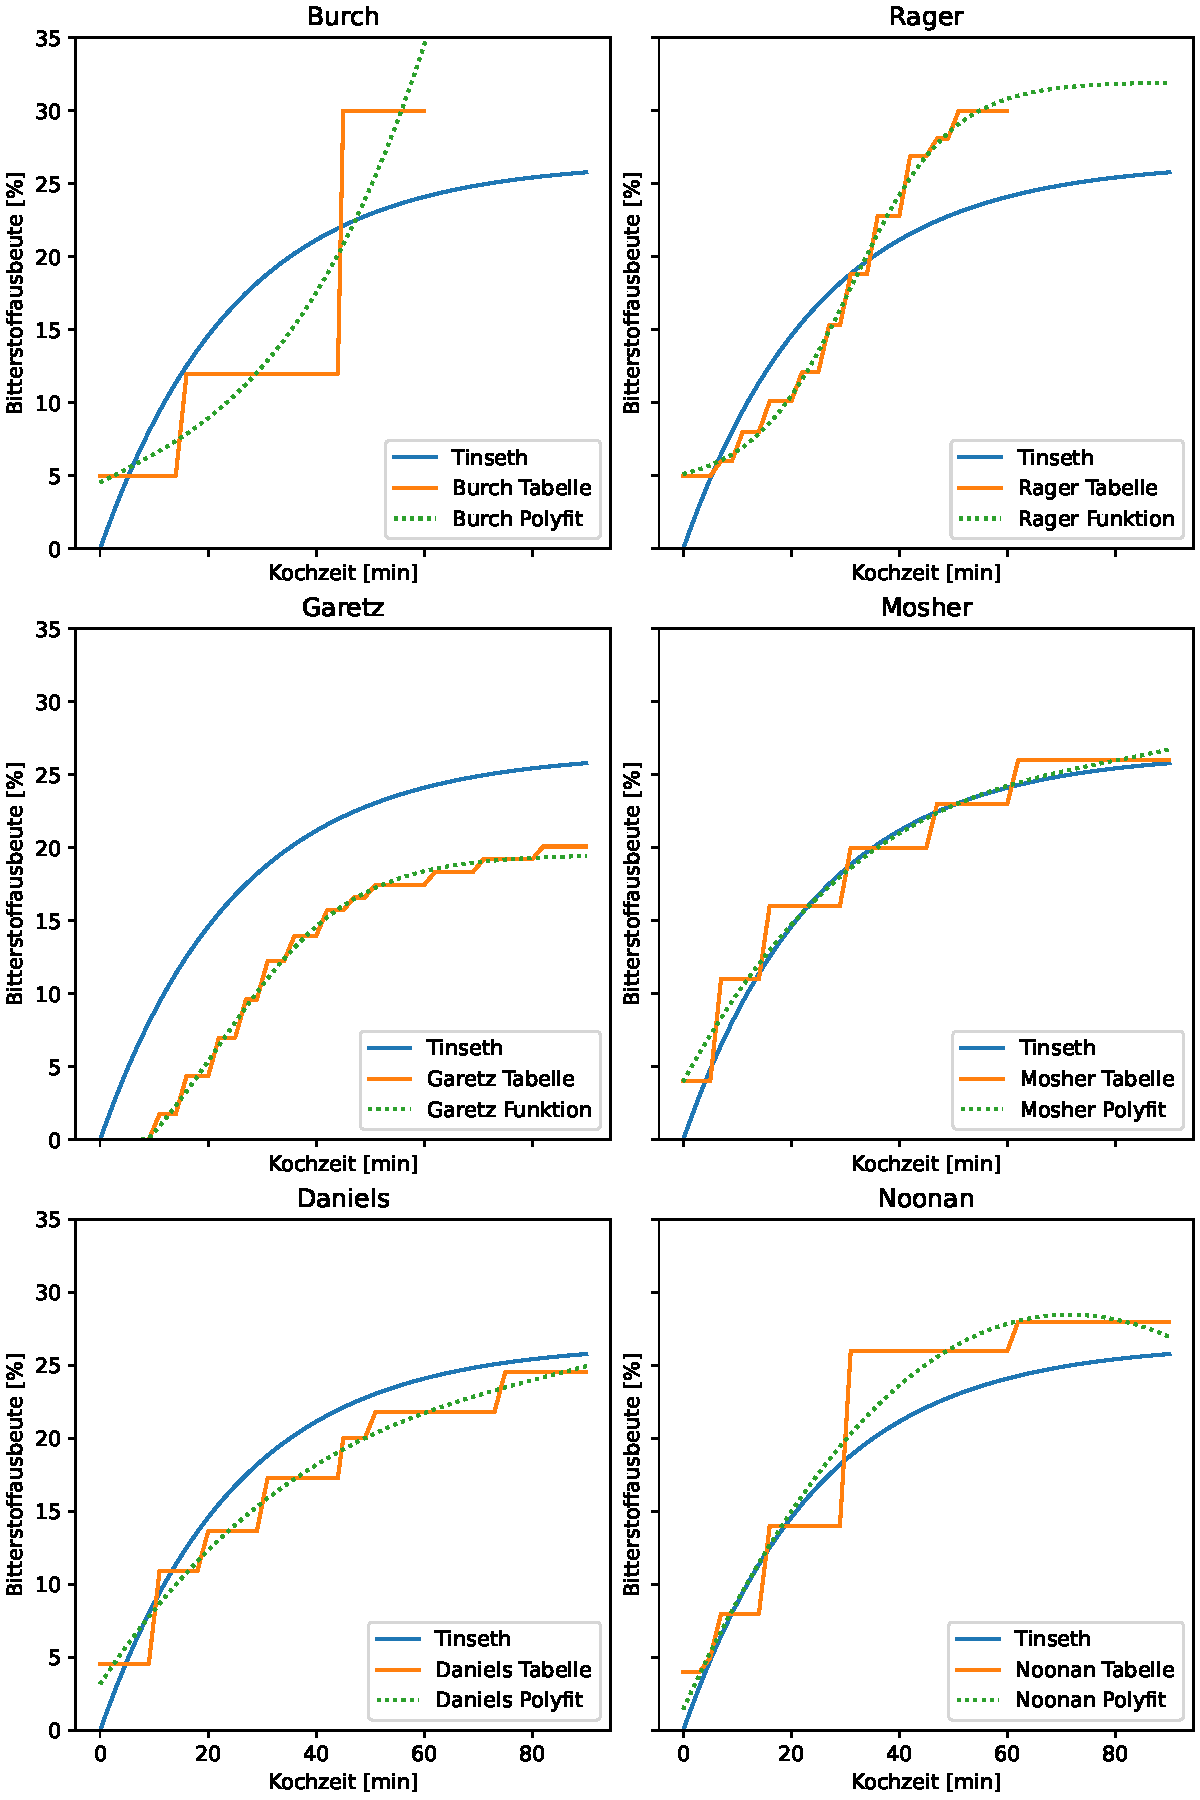
\includegraphics[width=14cm]{graph_utilization.pdf}
\caption{Bitterstoffausbeute bei 10,5 \%w/w Extrakt in Pfvw (Ascher, 2022)}
\label{fig:utilcompare}
\end{figure}

Alle relevanten Faktoren, die Einfluss auf die Bitterstoffausbeute nehmen, in ein praktikables Berechnungsverfahren zu integrieren, ist nahezu unmöglich. Dabei ist auch zu berücksichtigen, dass selbst der bekannte Alphasäuregehalt eines eingesetzten Hopfens aufgrund von Rohstoffschwankungen nicht dem realen Alphasäuregehalt entsprechen muss. Die zugrunde liegenden Messdaten für die verglichenen Modelle sind spezifisch für die Brausysteme, für die diese erhoben wurden. Tinseth schätzt, dass ein mit seinem Modell berechneter IBU-Wert im Idealfall innerhalb einer Abweichung von 10~\% vom realen Messwert liegt \parencite[22:05-23:00]{Smith2011}. Eine Empfehlung zum Umgang mit Modellen zur Schätzung der Bitterstoffausbeute ist daher, mehrere Biere mit zunehmender Bitterstoffgabe in einem IBU-Bereich von circa 15 bis 70~IBU mit dem eigenen Brausystem zu brauen und daran den sensorischen Eindruck zu kalibrieren \parencite{Beechum2017}.

Es sind nur wenige veröffentlichte Vergleichsdaten von gemessenen IBU-Werten eines Bieres und den berechneten Modellschätzungen verfügbar. \textcite{Hall1997} hat die Daten in \autoref{table:exphall} für ein American Pale Ale mit drei Hopfengaben während des Hopfenkochens ermittelt. \textcite{Bonham2001} berichtet von einem Gemeinschaftsexperiment des „Homebrew Digest“ in 2001 bei dem 33 Biere von verschiedenen Personen nach dem gleichen Rezept gebraut und dann labortechnisch analysiert wurden (\autoref{table:expbonham}). Nach der Eliminierung einiger Ausreißer lagen rund 80~\% der Messwerte innerhalb von 15~\% des Mittelwerts der Messwerte. Die Hälfte der Messwerte sogar innerhalb von 5~\%. Diese Streuung verdeutlicht, dass Unterschiede im Brauprozess und von Braugeräten einen relevanten Einfluss auf die Bitterstoffausbeute ausüben. \textcite{Beechum2017} führten später ebenfalls ein ähnliches Experiment durch. Dabei wurden jeweils mehrere American Pale Ales (32~IBU), American IPAs (58~IBU) und Double IPAs (76~IBU) nach gleichem Rezept gebraut, gemessen und mit dem durch das Tinseth Modell berechneten IBU-Wert verglichen. Beim American Pale Ale war eine mittlere absolute Abweichung von 4,5~IBU, beim American IPA von 7,4~IBU und beim Double IPA von 21,3~IBU zu beobachten. Eine höhere Stammwürze verursacht daher vermutlich eine höhere Abweichung vom Messwert. Auch Unterschiede in der Dauer der Würzekühlung dürften eine Rolle spielen. Inzwischen wird im Heimbraubereich schneller gekühlt als noch zur Zeit der Veröffentlichung des Tinseth Modells. Dies sollte insgesamt zu überhöhten Schätzungen der Bitterstoffausbeute führen.


\begin{table}[h]
\centering
\begin{tabular}{lr}
\toprule
\multicolumn{1}{c}{\textbf{Modell}} & \multicolumn{1}{c}{\textbf{IBU}} \\
\midrule
Messwert nach ASBC & 45,5 \\
Rager             & 57,8 \\
Garetz            & 24,1 \\
Mosher            & 35,7 \\
Daniels           & 46,5 \\
Noonan            & 53,2 \\
Tinseth           & 47,5 \\
\bottomrule
\end{tabular}
\caption{Modellvergleich für ein American Pale Ale \parencite{Hall1997}}
\label{table:exphall}
\end{table}

\begin{table}[h]
\centering
\begin{tabular}{lr}
\toprule
\multicolumn{1}{c}{\textbf{Modell}} & \multicolumn{1}{c}{\textbf{IBU}} \\
\midrule
Messwert nach ASBC (gemittelt) & 62,1 \\
Burch             & 45,6 \\
Rager             & 53,5 \\
Garetz            & 41,0 \\
Daniels           & 67,9 \\
Noonan            & 56,9 \\
Tinseth           & 48,0 \\
\bottomrule
\end{tabular}
\caption{Modellvergleich \parencite{Bonham2001}}
\label{table:expbonham}
\end{table}

\section*{Berechnungsbespiel}

Bei einem Kleinsud mit einer Pfannenvollwürzekonzentration von 10,5~\%w/w und 20 Litern kalter Anstellwürze  mit einer Stammwürze (Stw) von 12~°P erfolgen zwei Hopfengaben: 10~g Magnum T90~Pellets mit 16,4~\% Alphasäure 60~Minuten vor Kochende und 7~g Tradition T90~Pellets mit 6,6~\% Alphasäure 5 Minuten vor Kochende. Berechne die resultierende Isoalphasäurekonzentration mithilfe des Tinseth Modells. Unter der Anwendung von \autoref{eq:calcptosg}, \autoref{eq:tinsethba} und \autoref{eq:ibucalc} (für T90~Pellets ist die Bitterstoffausbeute mit 1,1 zu multiplizieren) ergibt sich folgender Berechnungsweg:

\begin{align*}
d_{Pfvw} \uden &= \frac{10,5}{258,6 - \frac{10,5}{258,2} \cdot 227,1} + 1 = 1,042 \\
d_{Stw} \uden &= \frac{12}{258,6 - \frac{12}{258,2} \cdot 227,1} + 1 = 1,048 \\
\overline{d_{\mathit{Kd}}} \uden &= \frac{d_{Pfvw} + d_{Stw}}{2} = 1,045 \\
\BA_{1} \uper &= \frac{1 - e^{\left(-0,04 \cdot 60 \right)}}{4,15} \cdot 100 \cdot 1,65 \cdot 0,000125^{\left(1,045 - 1 \right)} \cdot 1,1 = 26,5 \\
\IBU_{1} \ucon &= \frac{10 \cdot 1000 \cdot \frac{16,4}{100} \cdot \frac{26,5}{100}}{20} = 21,7 \\
\BA_{2} \uper &= \frac{1 - e^{\left(-0,04 \cdot 5 \right)}}{4,15} \cdot 100 \cdot 1,65 \cdot 0,000125^{\left(1,045 - 1 \right)} \cdot 1,1 = 5,3 \\
\IBU_{2} \ucon &= \frac{7 \cdot 1000 \cdot \frac{6,6}{100} \cdot \frac{5,3}{100}}{20} = 1,2 \\
\IBU \ucon &= \IBU_{1} + \IBU_{2} = 22,9
\end{align*}



\section*{Zusammenfassung}

Die relevanten Eckpunkte dieses Artikels sind:

\begin{itemize}
\item Die primären Bitterstoffe für das Bier liefert der Hopfen in Form der Alphasäuren. Damit diese in Lösung gehen, müssen die Alphasäuren während des Hopfenkochens zu Isoalphasäuren isomerisiert werden.
   
\item Die Kennzahl für den sensorischen Bittereindruck eines Bieres ist die International Bitterness Unit (IBU). Diese quantifiziert die Konzentration der Isoalphasäuren im Bier in Milligramm pro Liter. Gemessen wird die IBU entweder indirekt mit einem Spektralphotometer oder einer HPLC-Apparatur.

\item Nur ein Teil der während eines Brauvorgangs zugeführten Alphasäuren finden sich im fertigen Bier als Isoalphasäuren wieder. Einerseits ist die Isomerisierungsrate abhängig von verschiedenen Parametern des Brauprozesses, insbesondere der Kochdauer, anderseits gehen Isoalphasäuren auch nach dem Hopfenkochen verloren. Prozesstechnisch wird dieser Anteil in Prozent als Bitterstoffausbeute gemessen.

\item Sind die Bitterstoffausbeute des Brauprozesses und der Alphasäuregehalt eines Hopfens bekannt, lassen sich benötigte Hopfenmengen berechnen, um einen bestimmten IBU-Wert einzustellen.

\item Nachdem für den Heimbraubereich nach wie vor keine kostengünstigen Messgeräte zur Ermittlung der Bitterstoffausbeute verfügbar sind, haben sich verschiedene Modelle zur Schätzung der Bitterstoffausbeute etabliert. Das bekannteste davon ist das Tinseth Modell, welches allerdings nur für Dolden und Hopfengaben während des Kochens ausgelegt ist.
\end{itemize}

\printbibliography[title=Quellen]

\end{document}